% TikZ Decorations, Patterns, and Gradients
% Demonstrates: fill patterns, gradients, shadows, decorations, and opacity.
% Compile with: pdflatex main.tex

\documentclass[border=10pt]{standalone}
\usepackage{tikz}
\usetikzlibrary{
    patterns,
    patterns.meta,
    decorations.pathmorphing,
    decorations.markings,
    decorations.text,
    shadows,
    shadings,
}

\begin{document}
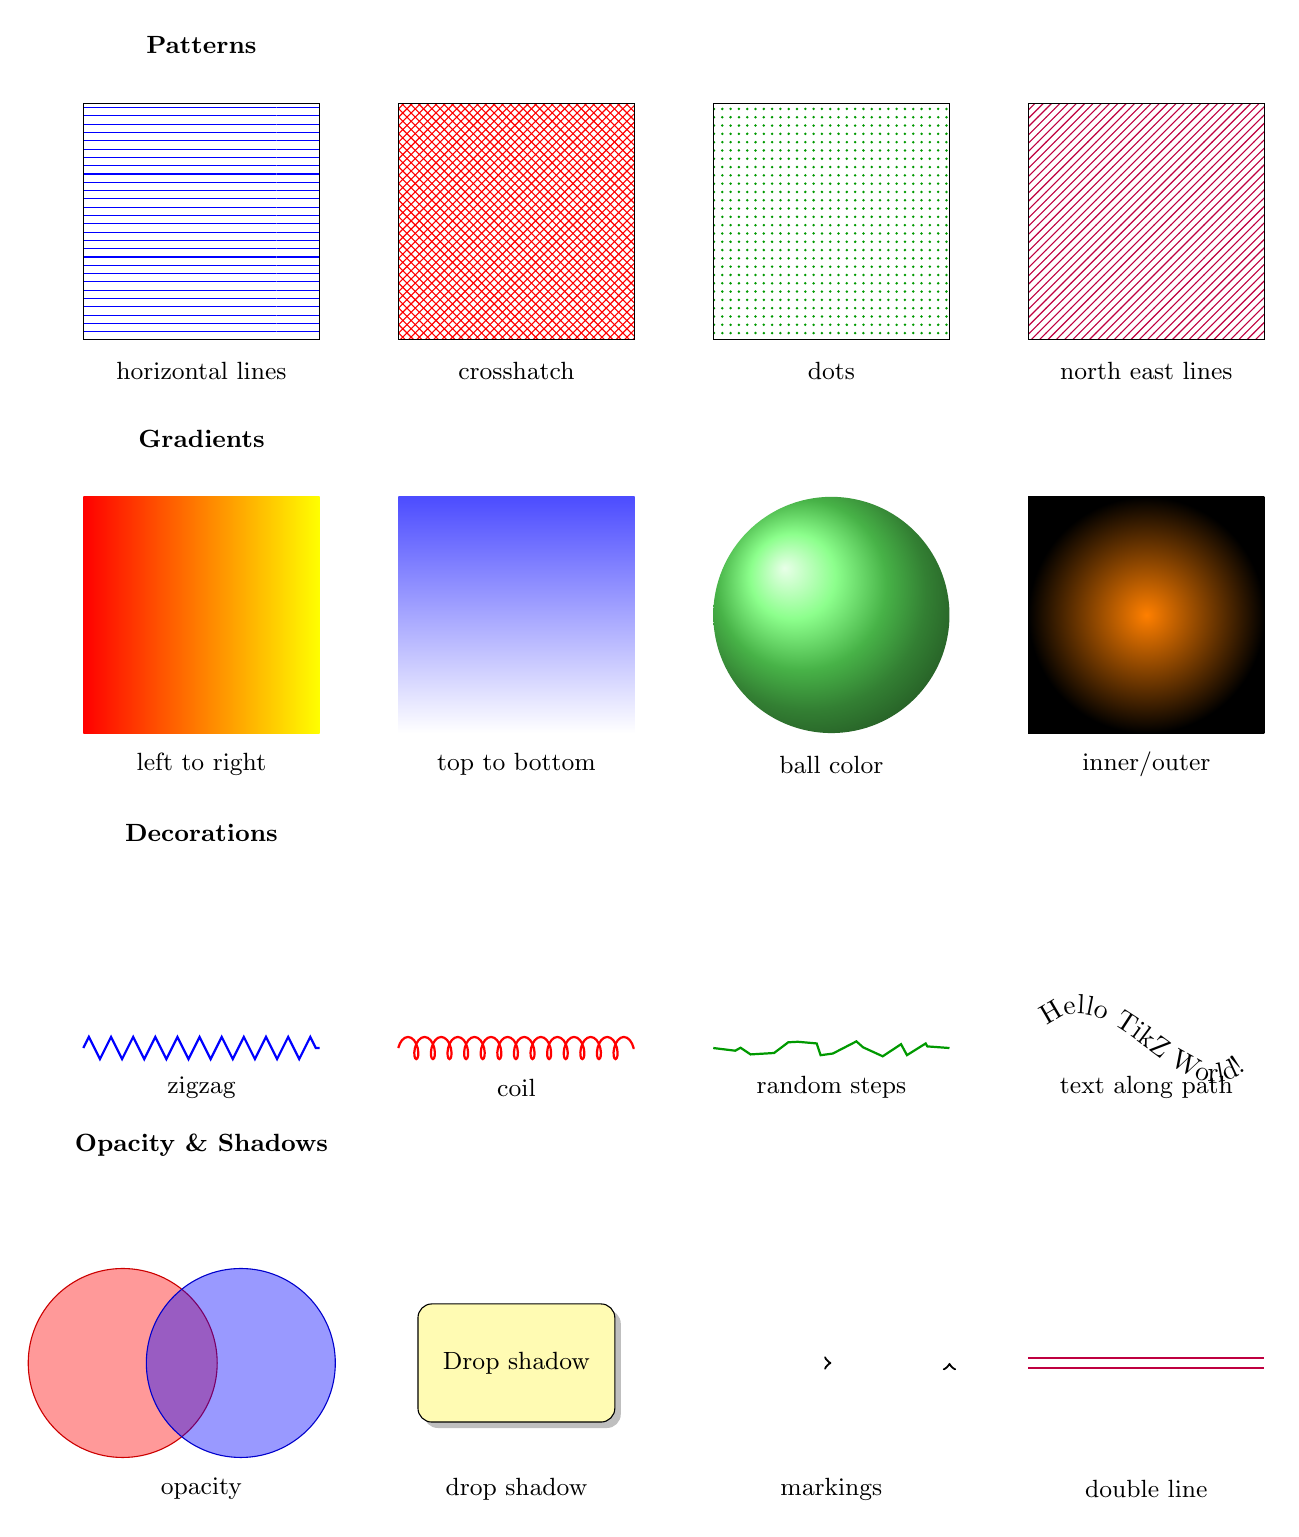
\begin{tikzpicture}[every node/.style={font=\small}]

% =============================================================================
% Row 1: Fill patterns
% =============================================================================
\node[anchor=south] at (1.5, 3.5) {\textbf{Patterns}};

% Horizontal lines pattern
\draw[pattern=horizontal lines, pattern color=blue]
    (0, 0) rectangle (3, 3);
\node at (1.5, -0.4) {horizontal lines};

% Crosshatch pattern
\draw[pattern=crosshatch, pattern color=red]
    (4, 0) rectangle (7, 3);
\node at (5.5, -0.4) {crosshatch};

% Dots pattern
\draw[pattern=dots, pattern color=green!60!black]
    (8, 0) rectangle (11, 3);
\node at (9.5, -0.4) {dots};

% North east lines
\draw[pattern=north east lines, pattern color=purple]
    (12, 0) rectangle (15, 3);
\node at (13.5, -0.4) {north east lines};

% =============================================================================
% Row 2: Gradients and shadings
% =============================================================================
\node[anchor=south] at (1.5, -1.5) {\textbf{Gradients}};

% Left-to-right gradient
\shade[left color=red, right color=yellow]
    (0, -5) rectangle (3, -2);
\node at (1.5, -5.4) {left to right};

% Top-to-bottom gradient
\shade[top color=blue!70, bottom color=white]
    (4, -5) rectangle (7, -2);
\node at (5.5, -5.4) {top to bottom};

% Radial (ball) shading
\shade[ball color=green!60]
    (9.5, -3.5) circle (1.5);
\node at (9.5, -5.4) {ball color};

% Custom inner/outer color
\shade[inner color=orange, outer color=black]
    (12, -5) rectangle (15, -2);
\node at (13.5, -5.4) {inner/outer};

% =============================================================================
% Row 3: Decorations
% =============================================================================
\node[anchor=south] at (1.5, -6.5) {\textbf{Decorations}};

% Snake (zigzag)
\draw[decorate, decoration={zigzag, amplitude=4pt, segment length=8pt},
      thick, blue]
    (0, -9) -- (3, -9);
\node at (1.5, -9.5) {zigzag};

% Coil / bumps
\draw[decorate, decoration={coil, amplitude=4pt, segment length=6pt},
      thick, red]
    (4, -9) -- (7, -9);
\node at (5.5, -9.5) {coil};

% Random steps
\draw[decorate, decoration={random steps, amplitude=3pt, segment length=5pt},
      thick, green!60!black]
    (8, -9) -- (11, -9);
\node at (9.5, -9.5) {random steps};

% Text along path
\draw[decorate, decoration={text along path,
      text={Hello TikZ World!}, text align=center},
      thick, purple]
    (12, -9) .. controls (13, -7.5) and (14, -10.5) .. (15, -9);
\node at (13.5, -9.5) {text along path};

% =============================================================================
% Row 4: Opacity and shadows
% =============================================================================
\node[anchor=south] at (1.5, -10.5) {\textbf{Opacity \& Shadows}};

% Overlapping transparent shapes
\filldraw[fill=red, fill opacity=0.4, draw=red!80!black]
    (0.5, -13) circle (1.2);
\filldraw[fill=blue, fill opacity=0.4, draw=blue!80!black]
    (2, -13) circle (1.2);
\node at (1.5, -14.6) {opacity};

% Drop shadow on a node
\node[draw, fill=yellow!30, rounded corners=5pt,
      drop shadow, minimum width=2.5cm, minimum height=1.5cm]
    at (5.5, -13) {Drop shadow};
\node at (5.5, -14.6) {drop shadow};

% Arrow with midpoint marking
\draw[->, thick,
      decorate, decoration={markings,
          mark=at position 0.5 with {\arrow{>}}}]
    (8, -13) -- (11, -13);
\node at (9.5, -14.6) {markings};

% Dashed + double line
\draw[double, double distance=3pt, thick, purple]
    (12, -13) -- (15, -13);
\node at (13.5, -14.6) {double line};

\end{tikzpicture}
\end{document}
